\chapter{Analyse}

\section{Recherche}

\subsubsection{Bezeichnung}
Der Ausdruck \gls{glos:droneLabel} kommt vom niederdeutschen Wort \textit{"`drone"'}, welches wiederrum seine Ursprung beim indogermanischen Wort \textit{"`dhren"'} hat. Die Bedeutung dieses Wortes lautet "`brummen"' oder "`dröhnen"'. \footcite{Geschichte_der_Drohne_-_Nachrichten_Print_-_DIE_WELT_-_Wissen_Print_DW_-_DIE_WELT_2015-03-21}

\begin{framed}
	\textit{Definition: }\textbf{\gls{glos:droneLabel}}\\
	Als \gls{glos:droneLabel} wird ein unbemanntes Luftfahrzeug bezeichnet. Die Steuerung kann entweder manuell oder autonom erfolgen.\footcite{Drone_Define_Drone_at_Dictionary.com_2015-03-21}
\end{framed}

\subsection{Geschichte der Drohne}
% http://www.informatik.uni-oldenburg.de/~iug08/snd/geschichte1.html
% http://diepresse.com/home/politik/innenpolitik/1385181/Die-Geschichte-der-Drohnen
% http://www.welt.de/print/welt_kompakt/print_lifestyle/article135929763/Kleine-Geschichte-der-Drohnen.html
% http://www.welt.de/print/die_welt/wissen/article127106535/Geschichte-der-Drohne.html
% http://de.wikipedia.org/wiki/Unbemanntes_Luftfahrzeug
% http://de.wikipedia.org/w/index.php?title=Autonomes_Luftfahrzeug&action=edit&redlink=1
% http://en.wikipedia.org/wiki/History_of_unmanned_aerial_vehicles

\subsection{Frühe Entwicklung}
Eine der allerersten bekannten \gls{glos:droneLabel} war wohl, 1783 von den Brüder Mongolfier aus Frankreich, ein unbemannter Heissluftballon. \footcite{Kleine_Geschichte_der_Drohnen_-_Nachrichten_Print_-_WELT_KOMPAKT_-_Lifestyle_-_DIE_WELT_2015-03-21}

\subsection{Militärische Zwecke}
Anschliessend wurde das Potenzial von \glspl{glos:droneLabel} besonders für kriegerische Zwecke erforscht und entwickelt.

\begin{wrapfigure}{r}{0.4\textwidth}
	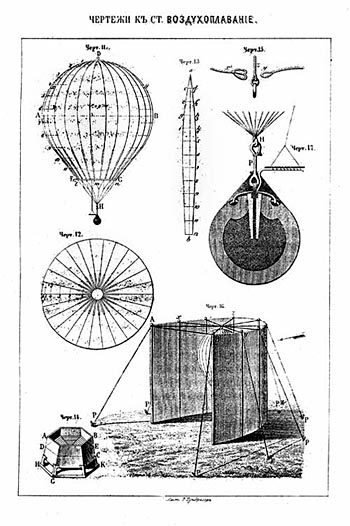
\includegraphics[width=1.0\linewidth]{images/analysis/balloonbombs1849.jpg}
	\caption[Bombing by Balloon, 1848]{Bombing by Balloon, 1848 \protect\footcite{Remote_Piloted_Aerial_Vehicles_2015-03-21}}
\end{wrapfigure}

So wurden bereits 1849, vom österreichischen Königsreich, unbemannte Heissluftballons mit Bomben im Krieg gegen Venedig losgeschickt.
Weder die "`\gls{glos:droneLabel}"' selbst, noch das Abwerfen der Bombe konnten aktiv gesteuert werden.
Die Heissluftballons flogen mit dem Wind und die Bomben wurde per Zeitzünder gezündet. Tatsächlich erreichten einzelne Ballons ihr Ziel und konnten Schaden anrichten, andere jedoch wurden vom Wind zurück geweht und zerstörten das eigene Territorium Österreichs. \footcite{Remote_Piloted_Aerial_Vehicles_2015-03-21}











\subsection{Flugeigenschaften von Drohnen}


\subsection{Bereits bestehende Arbeiten}

\subsubsection{Steuermöglichkeiten}

\subsubsection{Sensoren Integration auf bestehende Steuerungen}

%%% 

\section{Ist-Analyse}
\subsection{Gestensensor}

\subsubsection{Einsatz}

\subsubsection{Technische Details}

\subsubsection{API}


\subsection{Drohne}

\subsubsection{API}
% \subsubsection{Sensoren charakterisieren}

%%% 

\section{Soll-Analyse}
\subsection{Gesten-Steuerbeschrieb}


%%% 
